\documentclass[12pt]{extarticle}
\usepackage{geometry}
\geometry{
a4paper,
total={170mm,257mm},
left=20mm,
top=20mm,
headheight=12pt
}

\usepackage[parfill]{parskip} % Activate to begin paragraphs with an empty line rather than an indent
\usepackage{graphicx} % Use pdf, png, jpg, or eps§ with pdflatex; use eps in DVI mode
% TeX will automatically convert eps --> pdf in pdflatex
\graphicspath{ {./Figures/} }
\usepackage[labelfont=bf]{caption}
\usepackage{float}

\usepackage{amssymb,amsmath,amsthm}
\usepackage{commath}
\usepackage[hyphens]{url}
\usepackage[dvipsnames]{xcolor}
\usepackage[unicode=true,colorlinks=true,urlcolor=CadetBlue,citecolor=black,linkcolor=black]{hyperref}
\PassOptionsToPackage{hyphens}{url} % url is loaded by hyperref
\usepackage{authblk}
\usepackage{longtable}
\usepackage{multirow}
\usepackage{booktabs}
\usepackage{lipsum}  
\usepackage[title,page]{appendix}
\usepackage{chngcntr}
%\usepackage{endfloat}
      
%SetFonts
% newtxtext+newtxmath
\usepackage{newtxtext} %loads helv for ss, txtt for tt
\usepackage{amsmath}
\usepackage[bigdelims]{newtxmath}
\usepackage[T1]{fontenc}
\usepackage{textcomp}
%SetFonts

% less space before sections 
% https://tex.stackexchange.com/a/101126
\usepackage{titlesec}
\titlespacing*{\section}{0pt}{0.5\baselineskip}{0\baselineskip}
\titlespacing*{\subsection}{0pt}{0.5\baselineskip}{0\baselineskip}
    
% Species names
%% Meta-Command for defining new species macros
\usepackage{xspace}

\newcommand{\species}[3]{%
  \newcommand{#1}{\gdef#1{\textit{#3}\xspace}\textit{#2}\xspace}}
  
\species{\yeast}{Saccharomyces cerevisiae}{S.~cerevisiae}
\species{\calbicans}{Candida albicans}{C.~albicans}
\species{\cneoformans}{Cryptococcus neoformans}{C.~neoformans}

% line numbers
\usepackage[displaymath, mathlines]{lineno}
\renewcommand\linenumberfont{\normalfont\small\sffamily}
\linenumbers
\modulolinenumbers[2]

% Yoav & Lee commands
\newcommand*{\tr}{^\intercal}
\let\vec\mathbf
\newcommand{\matrx}[1]{{\Big[ \stackrel{}{#1}\Big]}}
\newcommand{\diag}[1]{\mbox{diag}\matrx{#1}}
\newcommand{\goesto}{\rightarrow}
\newcommand{\dspfrac}[2]{\frac{\displaystyle #1}{\displaystyle #2} }
\newtheorem{theorem}{Theorem}
\newtheorem{corollary}{Corollary}
\newtheorem{lemma}{Lemma}
\newtheorem{remark}{Remark}
\newtheorem{result}{Result}
\renewcommand\qedsymbol{} % no square at end of proof
\newcommand{\cl}{\mathbf{L}}
\newcommand{\cj}{\mathbf{J}}
\newcommand{\ci}{\mathbf{I}}
\DeclareMathOperator{\sign}{sign}

% Supplementary
% https://support.authorea.com/en-us/article/how-to-create-an-appendix-section-or-supplementary-information-1g25i5a/
\newcommand{\beginsupplement}{%
      	\setcounter{table}{0}
        \renewcommand{\thetable}{S\arabic{table}}%
        \setcounter{figure}{0}
        \renewcommand{\thefigure}{S\arabic{figure}}%
		\setcounter{equation}{0}
        \renewcommand{\theequation}{A\arabic{equation}}%
}

% autoref
\def\equationautorefname{Eq.}

% NatBib
\usepackage[numbers,square,comma,sort]{natbib}

% Title page
\title{Non-Vertical Cultural Transmission, Assortment, \\and the Evolution of Cooperation}

% Authors
\renewcommand\Affilfont{\small}

\author[1]{Dor Cohen}
\author[2]{Ohad Lewin-Epstein}
\author[3]{Marcus W. Feldman}
\author[1,4,5,*]{Yoav Ram}

\affil[1]{School of Computer Science, Interdisciplinary Center Herzliya, Herzliya, Israel}
\affil[2]{School of Plant Sciences and Food Security, Faculty of Life Sciences, Tel Aviv University, Tel Aviv, Israel}
\affil[3]{Department of Biology, Stanford University, Stanford, CA}
\affil[4]{School of Zoology, Faculty of Life Sciences, Tel Aviv University, Tel Aviv, Israel}
\affil[5]{Sagol School of Neuroscience, Tel Aviv University, Tel Aviv, Israel}
\affil[*]{Corresponding author: yoav@yoavram.com}

\date{\today}

\begin{document}
\maketitle

\section*{\huge{Supplementary material}}
\beginsupplement % https://support.authorea.com/en-us/article/how-to-create-an-appendix-section-or-supplementary-information-1g25i5a/

%%%%%%%%%%%%%%%%%%%%%%%%%%%%%%%%%%%%%%%%%%%%%%%%%%%%%%

%%% Figure: Invasion
\begin{figure}[h]
  \centering
  \includegraphics[width=1\textwidth]{PRSB_figures/fig_s1.pdf}
  \caption{
  \textbf{Reduction principle for interaction-transmission association.} 
  Consecutive fixation of modifier alleles that reduce interaction-transmission association $\alpha$ in numerical simulations of evolution with two modifier alleles (Eq.~D1).
  When an invading modifier allele is established in the population (frequency > 99.95\%), a new modifier allele that reduces interaction-transmission association by 5\% is introduced (at initial frequency 0.5\%).
  \textbf{(a)}~The frequency of the cooperative phenotype $A$ over time.
  \textbf{(b)}~The frequency of the invading modifier allele $m$ over time. 
  \textbf{(c)}~The population mean fitness ($\bar{w}$) over time.
  Here, $c = 0.05$, $b=1.3$, $T_A=0.4<T_B=0.7$, initial interaction-transmission association $\alpha_1=0.7$, lower interaction-transmission association threshold $a_2=0.605$.  
  }
  \label{fig:invasion}
\end{figure}



%%% Figure: Spatial model - local selection
\begin{figure}[h]
  \centering
  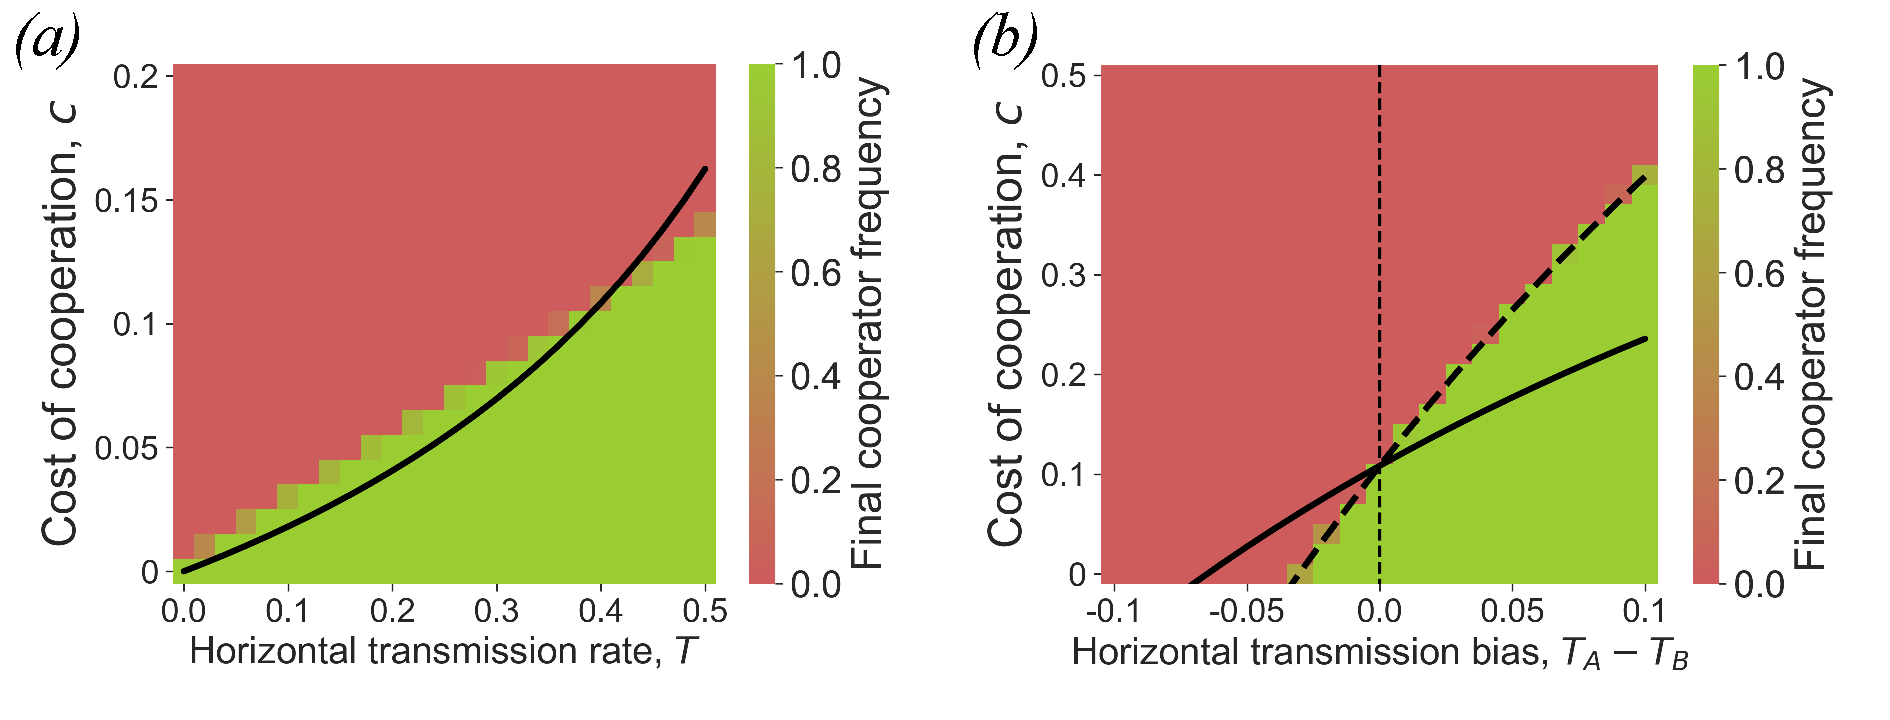
\includegraphics[width=1\textwidth]{PRSB_figures/fig_s2.pdf}
  \caption{
  \textbf{Evolution of cooperation in a structured population with local selection.}
  The expected frequency of cooperators in a structured population after 10,000 generations is shown (red for 0\%, green for 100\%) as a function of both the cost of cooperation ($c$) on the y-axis, and the symmetric horizontal transmission rate ($T=T_A=T_B$) on the x-axis of panel~\textbf{(a)}, or the transmission bias $T_A-T_B$ on the x-axis of panel~\textbf{(b)}.
  Cooperation and horizontal transmission are both local between neighbouring sites, and each site had 8 neighbours.
  Selection operates locally (see Figure 4 for results from a model with global selection).
  The black curves represent the cost thresholds for the evolution of cooperation in a well-mixed population with interaction-transmission association, where $\alpha=1/8$ in inequality~14 for panel~\textbf{(a)} and in Eqs.~12 for panel~\textbf{(b)}.
  The population evolves on a 100-by-100 grid.
  Simulations were stopped at generation 10,000 or if one of the phenotypes fixed.
  50 simulations were executed for each parameter set.
  Here, benefit of cooperation, $b=1.3$; perfect vertical transmission $v=1$.
  \textbf{(a)} Symmetric horizontal transmission, $T=T_A=T_B$.
  \textbf{(b)} Horizontal transmission rate $T_A$ is fixed at $0.4$, and $T_B$ varies, $0.3<T_B<0.5$.
  }
  \label{fig:spatial_local_selection}
\end{figure}



%%%
\end{document}